\documentclass[10pt]{article}

\usepackage{enumerate,graphicx}
\usepackage{hyperref}
\usepackage{amsmath}
\usepackage{amssymb}
\usepackage{graphicx}
\usepackage{caption}
\usepackage{subfig}
\usepackage{subcaption}
\usepackage{array,multirow,graphicx}
\usepackage{titlesec}

% \titleformat{\section}
%   {\normalfont\fontsize{12}{15}\bfseries}{\thesection}{1em}{}

\usepackage[
    backend=biber,
    style=authoryear,
  ]{biblatex}

\addbibresource{report.bib}

\pagestyle{empty}

\title{Computer Vision Summative Assignment}
\author{hfsk44}
\date{\today}
 
\begin{document}
 
\maketitle

\section *{Preprocessing}

\subsection *{Downsampling}
    All input images are first downsampled to a specified quality. This decrease in image size results in a significant performance improvement at the expense of some minor loss in accuracy. The upper 150 pixels are cropped out as they are highly unlikely to contain road, saving roughly 0.9s per frame.

    \begin{figure}[!h]
        \centering
        \subfloat[quality=1 time=3.92s]{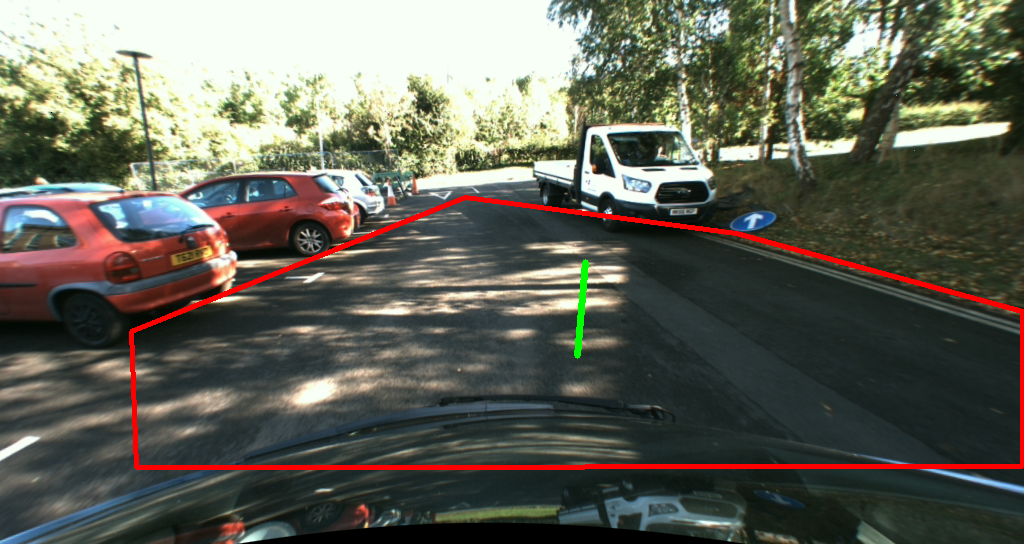
\includegraphics[width=0.4\textwidth]{ds100_3x92.png}\label{fig:f1}}
        \hfill
        \subfloat[quality=0.75 time=2.08s]{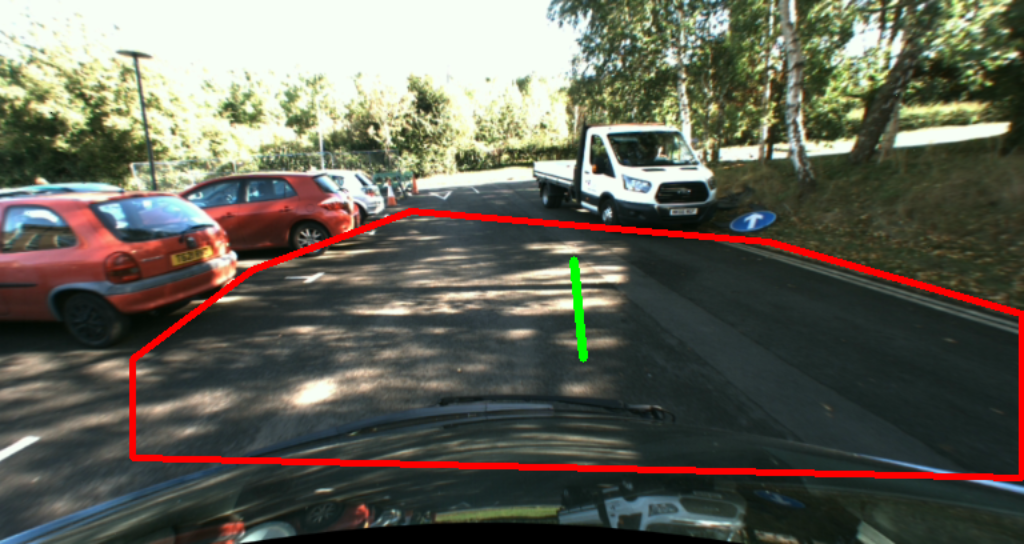
\includegraphics[width=0.4\textwidth]{ds75_2x08.png}\label{fig:f2}}
        \\
        \subfloat[quality=0.50 time=1.10s]{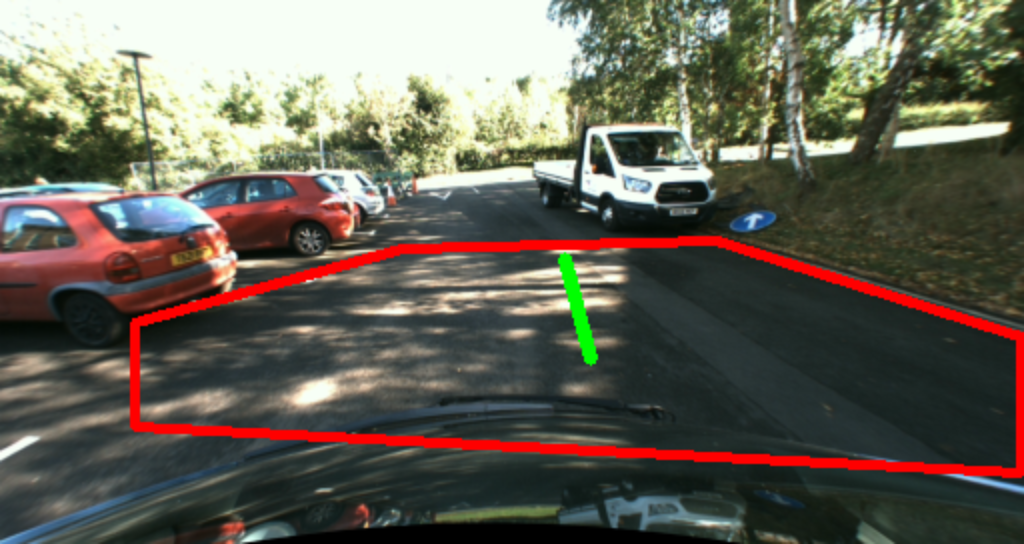
\includegraphics[width=0.4\textwidth]{ds50_1x10.png}\label{fig:f2}}
        \hfill
        \subfloat[quality=0.25 time=0.61s]{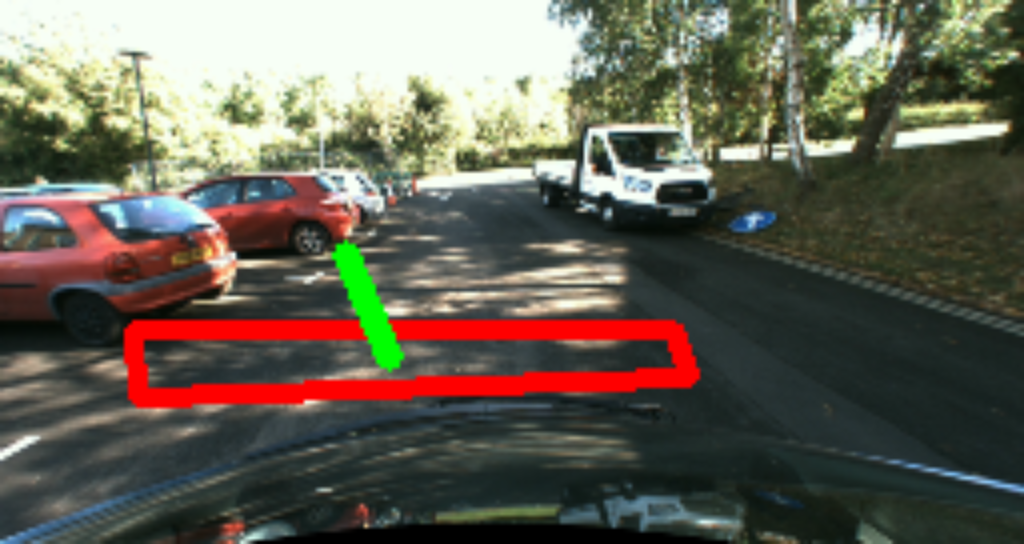
\includegraphics[width=0.4\textwidth]{ds25_0x61.png}\label{fig:f2}}
        \caption{Results of downsampling at different rates}
    \end{figure}

\newpage

\subsection *{HSV Masking}
    Input from the left camera is converted to HSV and thresholded for values within the range $(40,60,60) \rightarrow (80,255,255)$ i.e. different levels of green. This resulted in a highly effective mask for removing grass and trees. Other objects such as cobbles would also fall in this range but in practice this would rarely affect results.

    \begin{figure}[!h]
        \centering
        \subfloat[With mask]{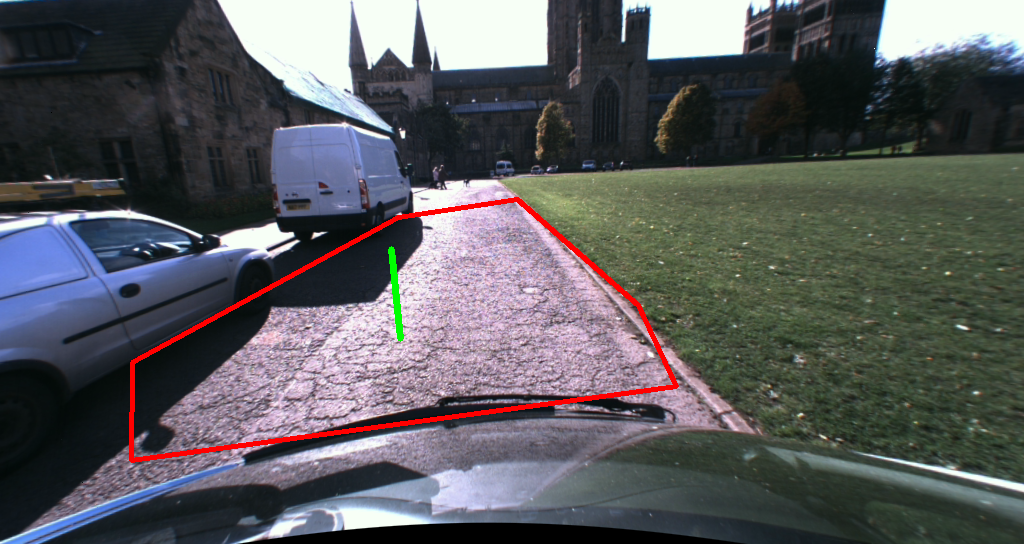
\includegraphics[width=0.4\textwidth]{green.png}\label{fig:f1}}
        \hfill
        \subfloat[Without mask]{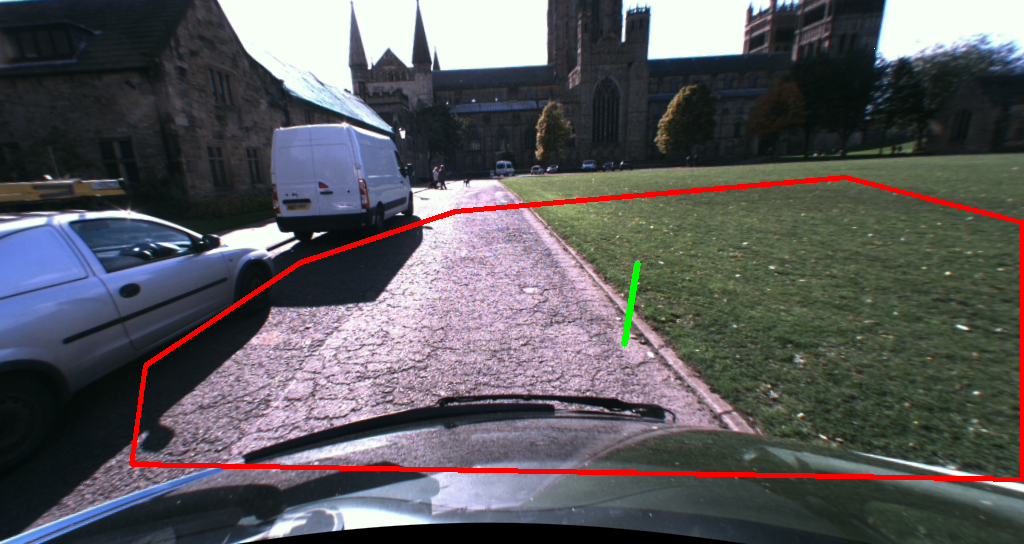
\includegraphics[width=0.4\textwidth]{nogreen.png}\label{fig:f2}}
        \hfill
        \subfloat[The mask itself]{
\includegraphics[width=0.4\textwidth]{greenmask.png}\label{fig:f2}}
        \hfill
        \subfloat[Cobbles erroneously detected as green]{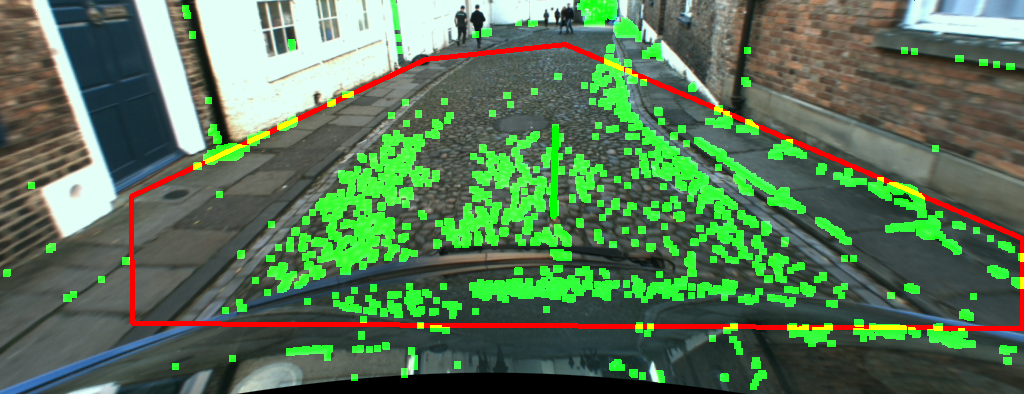
\includegraphics[width=0.4\textwidth]{greenerror.png}\label{fig:f2}}

        \caption{Example of HSV masking in use}
    \end{figure}

\subsection *{Edge Masking}
    The result of a canny on the left image is used to create a mask for splitting consensus points that are separated by a strong edge. This is often effective in separating the road region from pavement and cars. The central region of the canny image is masked out in order to prevent road markings from separating the road region.

    \begin{figure}[!h]
        \centering
        \subfloat[With mask]{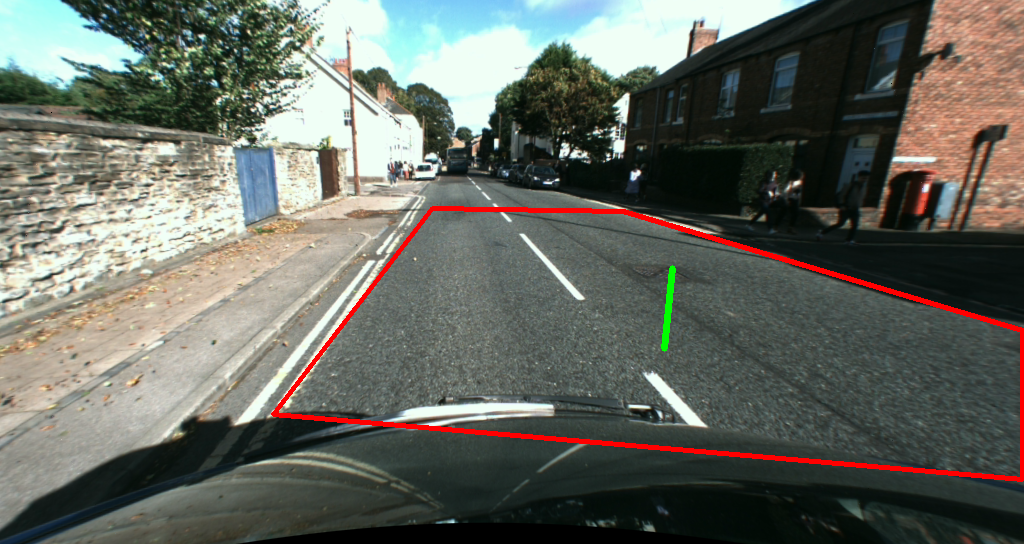
\includegraphics[width=0.4\textwidth]{canny.png}\label{fig:f1}}
        \hfill
        \subfloat[Without mask]{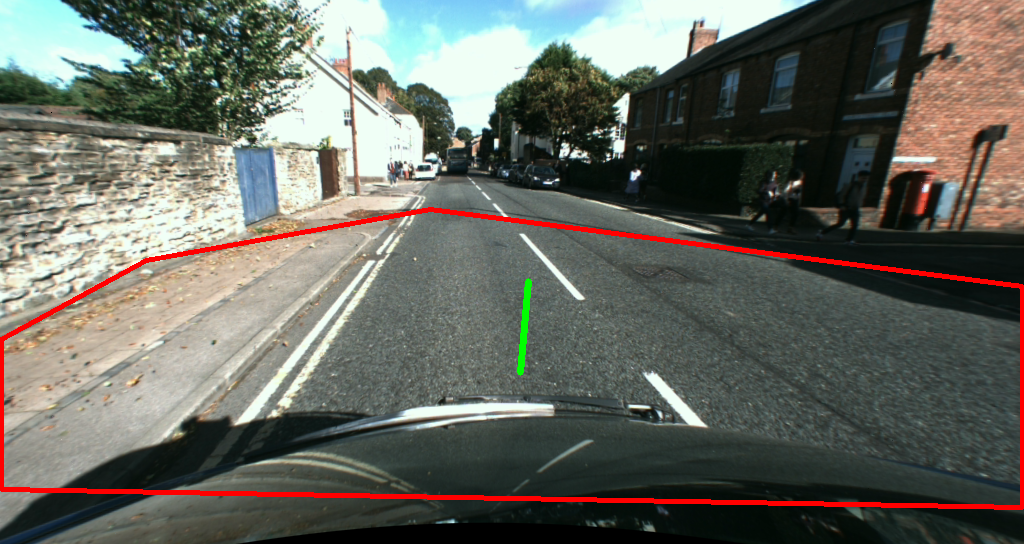
\includegraphics[width=0.4\textwidth]{nocanny.png}\label{fig:f2}}
        \hfill
        \subfloat[The mask itself]{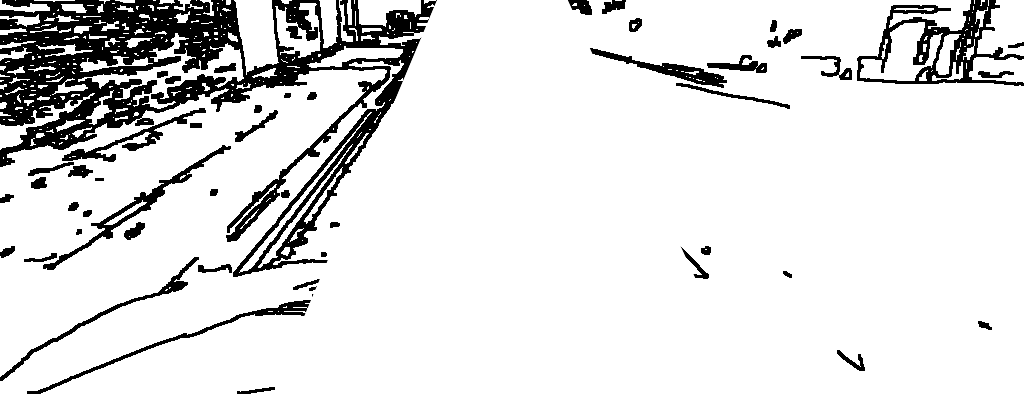
\includegraphics[width=0.4\textwidth]{cannymask.png}\label{fig:f2}}
        \hfill
        \subfloat[Mask used to ignore center region]{
\includegraphics[width=0.4\textwidth]{cannymaskmask.png}\label{fig:f2}}

        \caption{Example of edge masking in use}
    \end{figure}
\newpage

\subsection *{Contrast Stretching}
    When calculating disparity, pixel values of the greyscale input images are raised to the power $0.75$. This helps prevent sharp changes in disparity along the edge of shadows on the road surface.

    \begin{figure}[!h]
        \centering
        \subfloat[With contrast stretching]{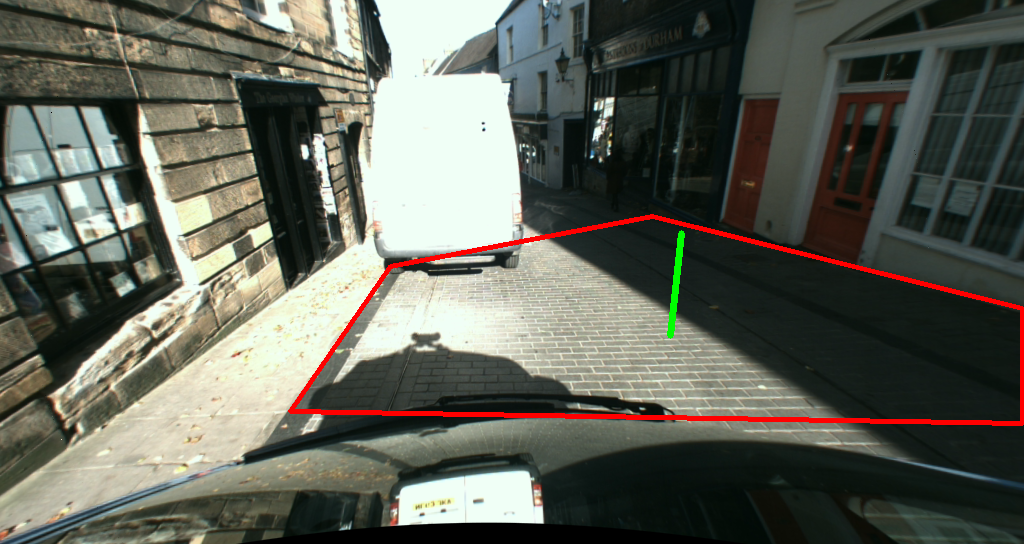
\includegraphics[width=0.4\textwidth]{withgamma.png}\label{fig:f1}}
        \hfill
        \subfloat[Without contrast stretching]{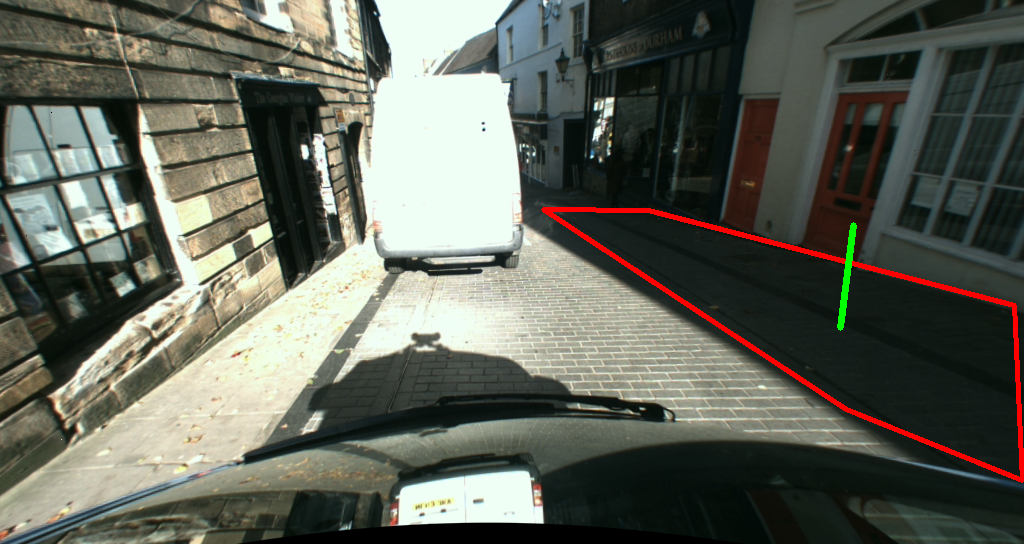
\includegraphics[width=0.4\textwidth]{withnogamma.png}\label{fig:f2}}
        \hfill
        \subfloat[With contrast stretching]{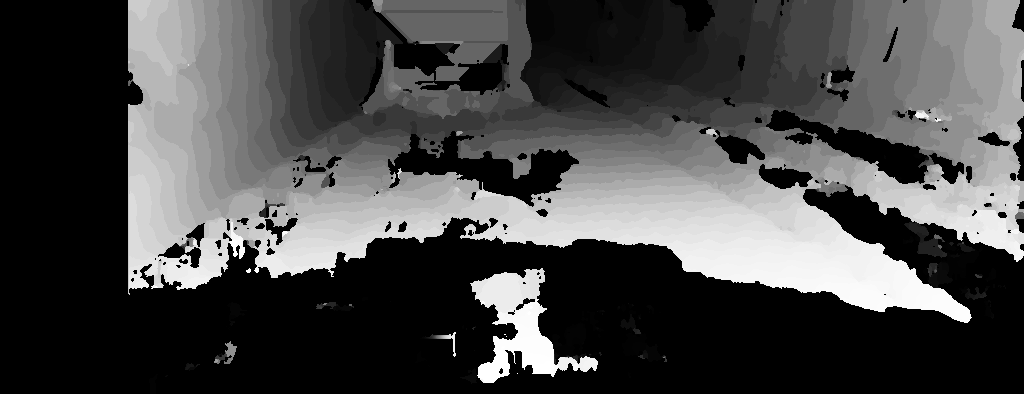
\includegraphics[width=0.4\textwidth]{withgammadisp.png}\label{fig:f2}}
        \hfill
        \subfloat[Without contrast stretching]{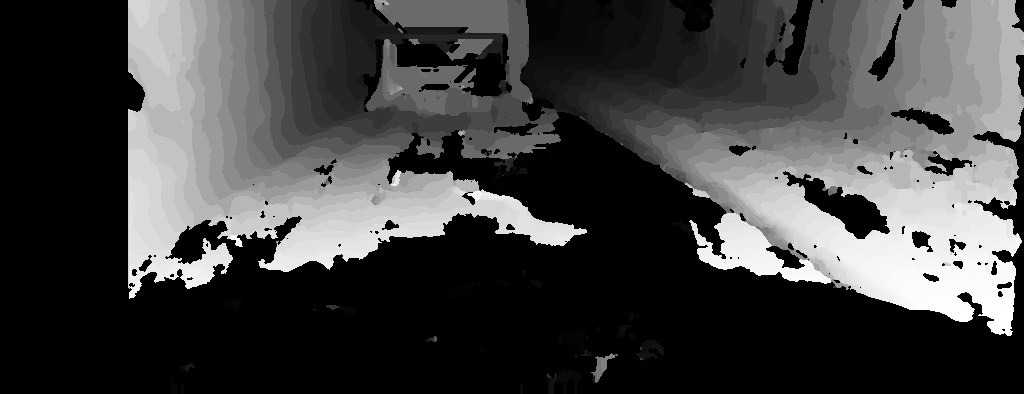
\includegraphics[width=0.4\textwidth]{withnogammadisp.png}\label{fig:f2}}

        \caption{Example of contrast stretching in use}
    \end{figure}

\newpage

\subsection *{Disparity Cleanup}
    Navier-Stokes inpainting is used to fill holes in the disparity image, improving results significantly as the majority of these holes occur on the road surface. Motion blur will often create sharp spikes in disparity, preventing a good plane from being found. Filtering out disparity values above 50 eliminates this issue. A pre-defined mask is applied to remove areas that are highly likely to not be a road e.g. sky and the car bonnet.

    \begin{figure}[!h]
        \centering
        \subfloat[With infilling]{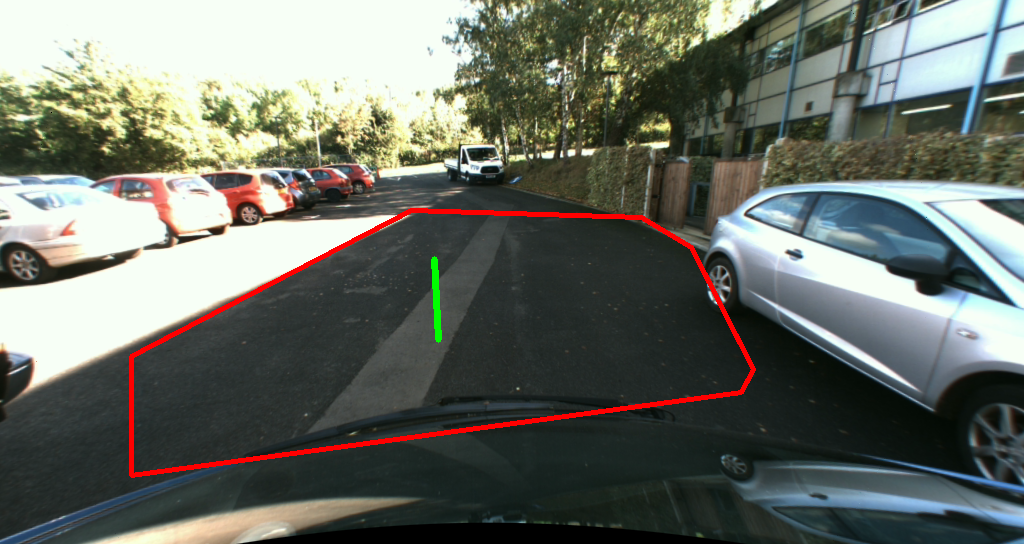
\includegraphics[width=0.4\textwidth]{disparityclean.png}\label{fig:f1}}
        \hfill
        \subfloat[Without infilling]{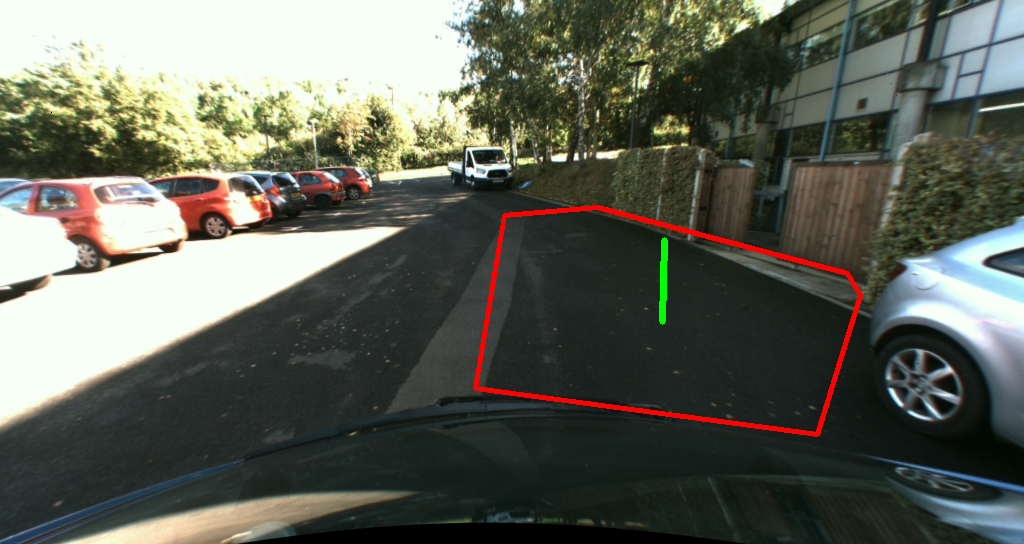
\includegraphics[width=0.4\textwidth]{disparitydirty.png}\label{fig:f2}}
        \\
        \subfloat[Infilled disparity]{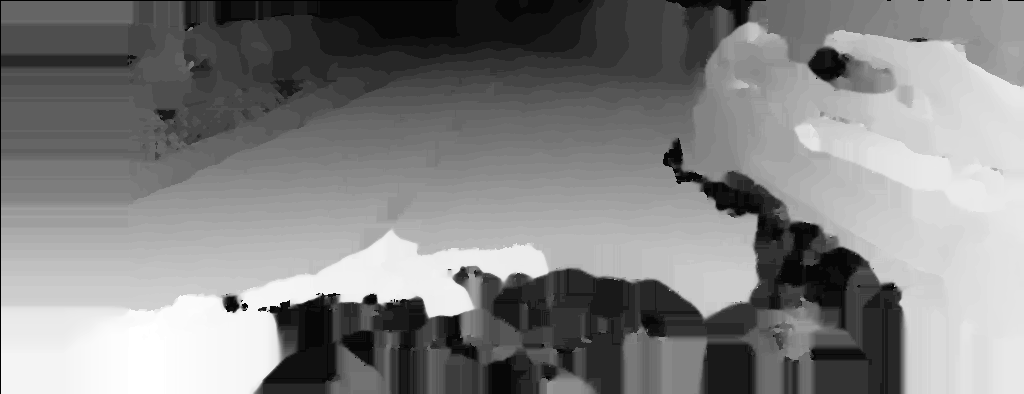
\includegraphics[width=0.4\textwidth]{filleddisparity.png}\label{fig:f2}}
        \hfill
        \subfloat[Raw disparity]{
\includegraphics[width=0.4\textwidth]{disparity.png}\label{fig:f2}}
        \caption{Example of disparity infilling in use}
    \end{figure}

    \begin{figure}[!h]
        \centering
        \subfloat[With filtering]{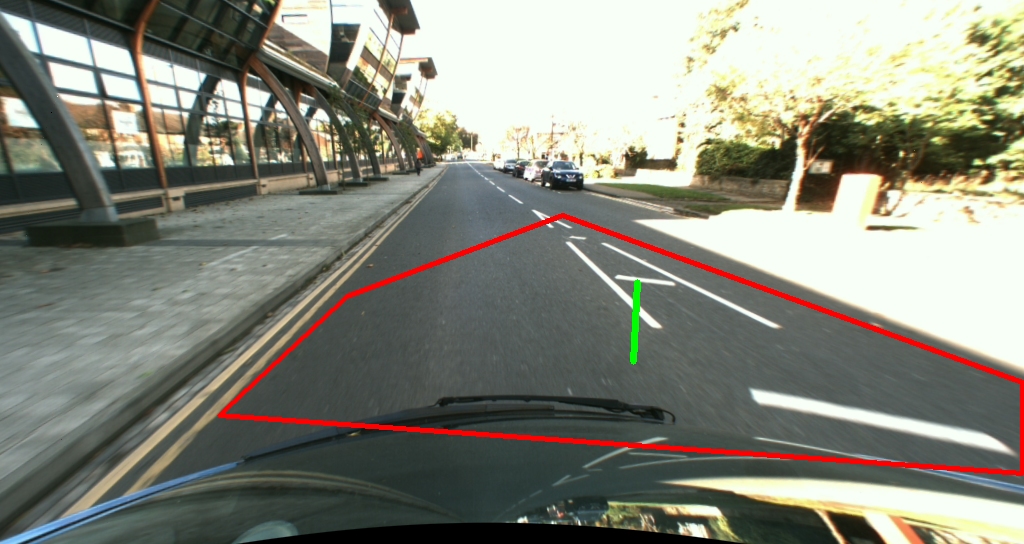
\includegraphics[width=0.4\textwidth]{spuriousfilteres.png}\label{fig:f1}}
        \hfill
        \subfloat[Without filtering]{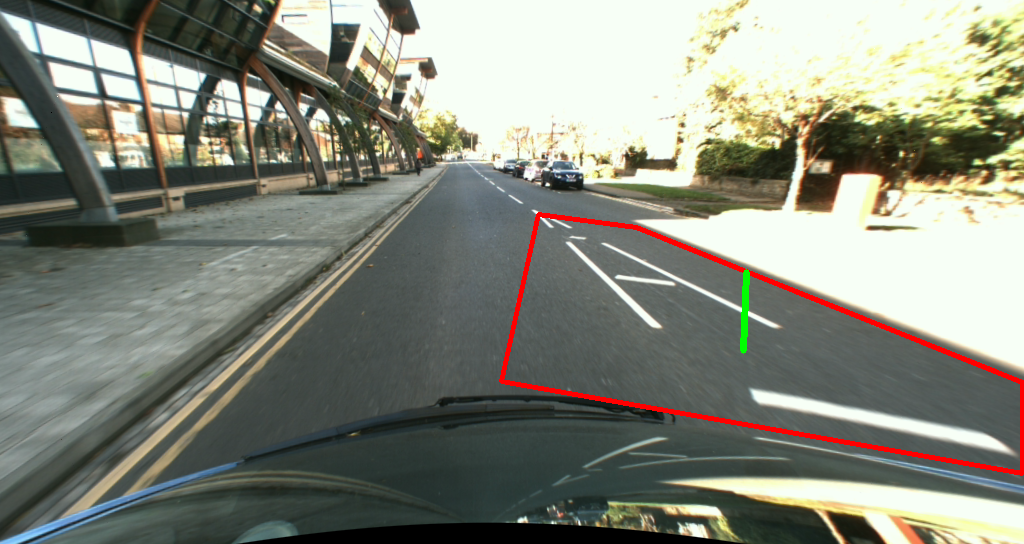
\includegraphics[width=0.4\textwidth]{spuriousunfilteres.png}\label{fig:f2}}
        \\
        \subfloat[Filtered disparity]{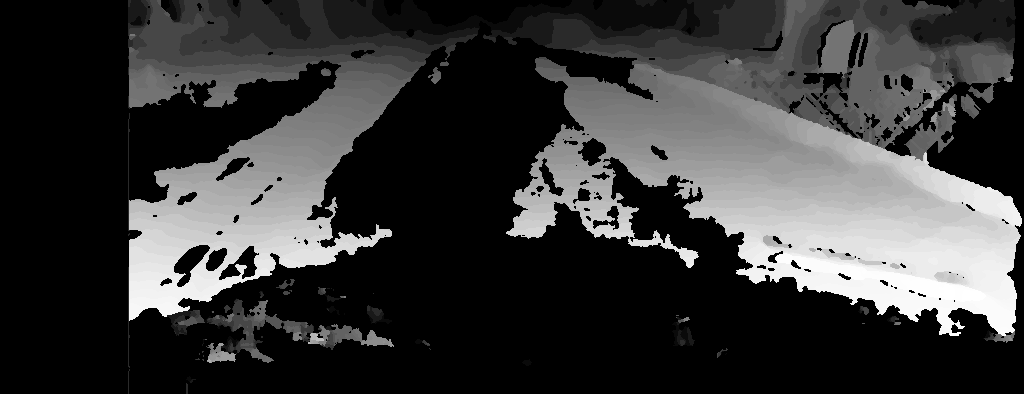
\includegraphics[width=0.4\textwidth]{spuriousfilter.png}\label{fig:f2}}
        \hfill
        \subfloat[Unfiltered disparity]{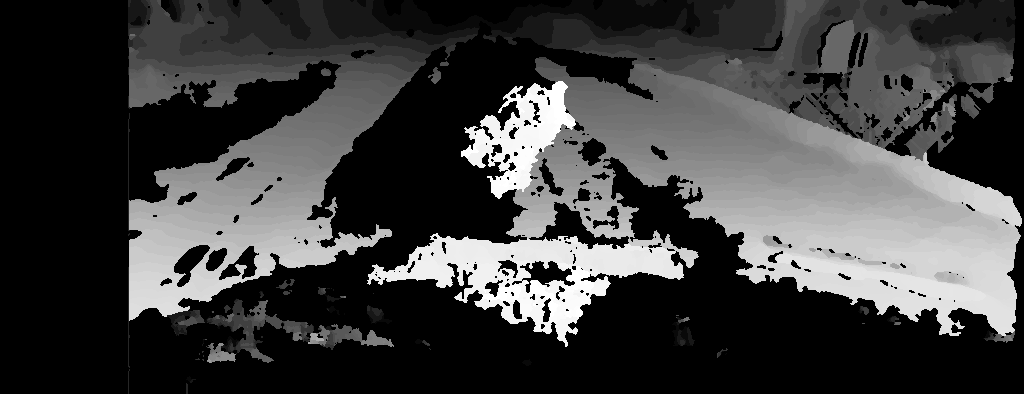
\includegraphics[width=0.4\textwidth]{spuriousunfilter.png}\label{fig:f2}}
        \caption{Example of high disparity value filtering in use}
    \end{figure}

\newpage
\section *{3D RANSAC}
    
\subsection *{Disparity Projection}
    Within the projection from disparity values to 3D points, the Z value is used as a coefficient in the calculations for X and Y instead of Zmax. This gives a smoother distribution of points in the Z axis, increasing the chance of finding a large plane significantly.

    \begin{figure}[!h]
        \centering
        \subfloat[Using Z]{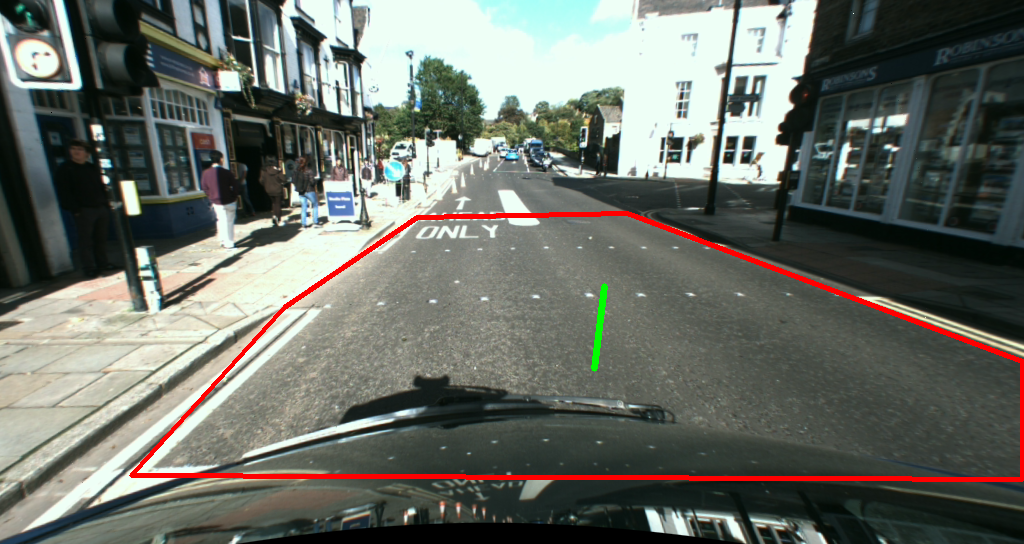
\includegraphics[width=0.4\textwidth]{zmax.png}\label{fig:f1}}
        \hfill
        \subfloat[Using Zmax]{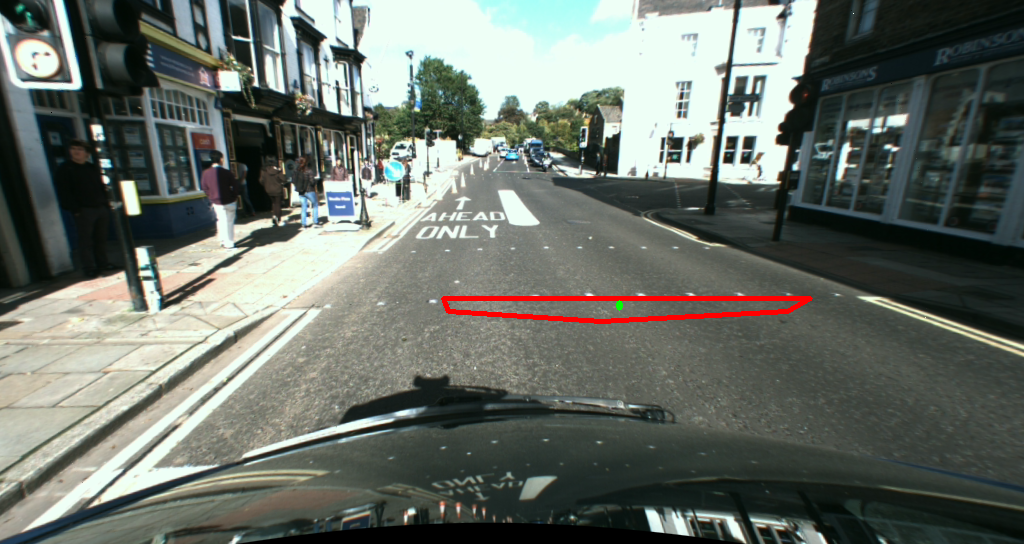
\includegraphics[width=0.4\textwidth]{z.png}\label{fig:f2}}
        \\
        \subfloat[Using Z]{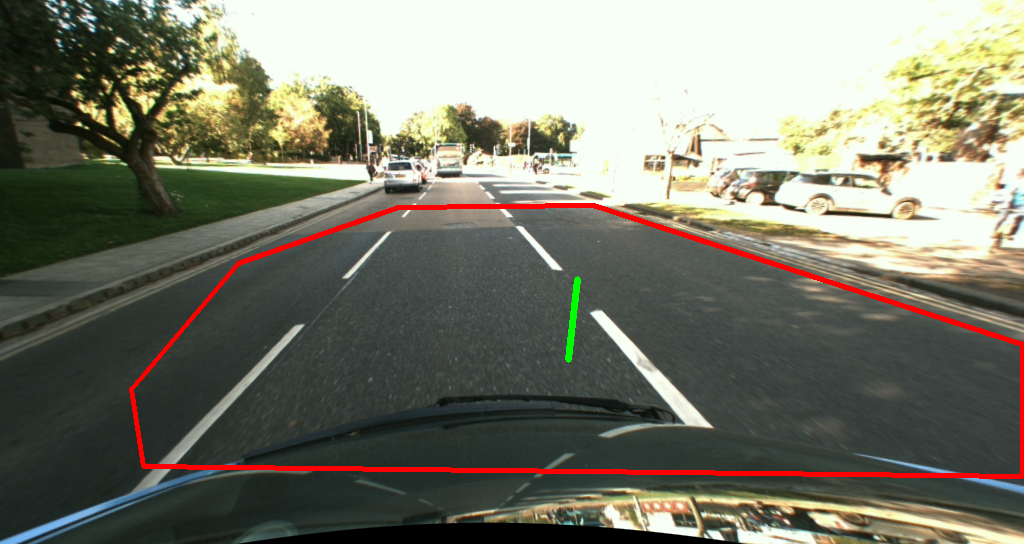
\includegraphics[width=0.4\textwidth]{zmax1.png}\label{fig:f1}}
        \hfill
        \subfloat[Using Zmax]{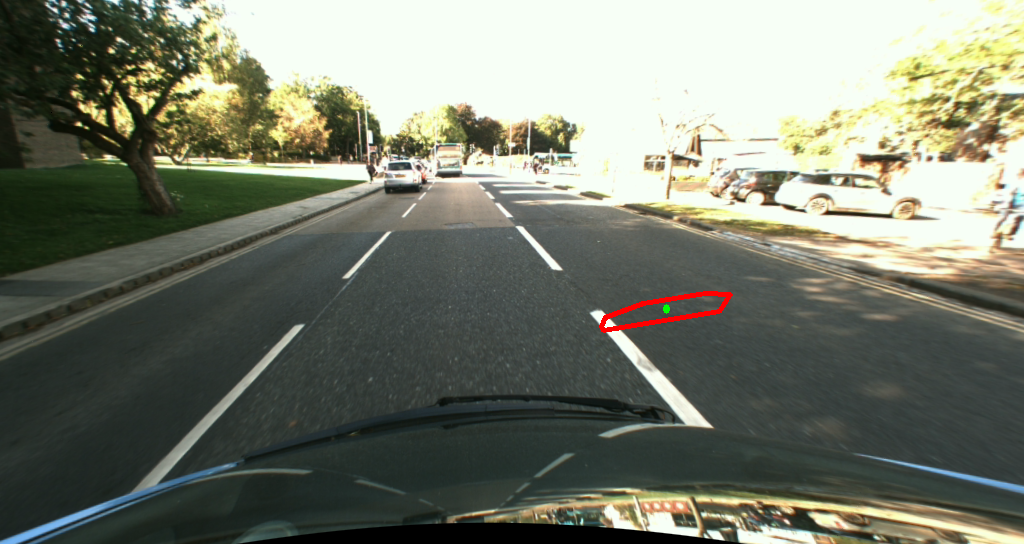
\includegraphics[width=0.4\textwidth]{z1.png}\label{fig:f2}}
        \caption{Results of using Z instead of Zmax}
    \end{figure}

\subsection *{RANSAC}
    200 iterations of a 3D RANSAC are performed, where the consensus points are those within a distance of 0.1 from the randomly chosen plane. The plane with the highest number of consensus points is taken to be the best estimate. \\
    Any plane with a $y$ coefficient less than 0.5 is immediately rejected, this is effective in preventing vertical planes such as the sides of cars and houses from being considered. \\
    After all 200 iterations have been performed, an average is taken between the best plane found for the current frame and its predecessor. If there are more consensus points to the average plane then it is returned instead. This often results in a slight improvement in results for the equivalent of one more RANSAC iteration.

    \begin{figure}[!h]
        \centering
        \subfloat[With y coefficient rejection]{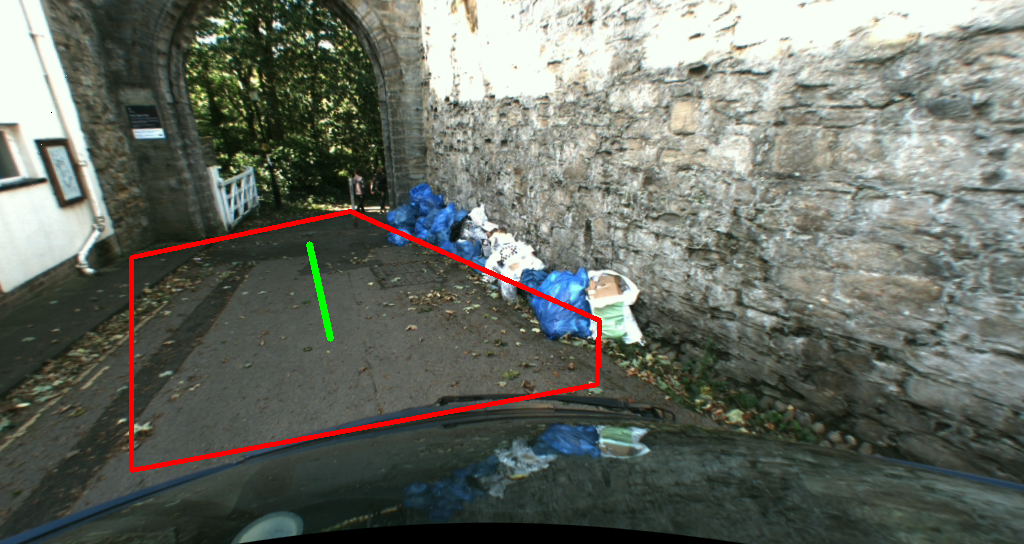
\includegraphics[width=0.4\textwidth]{b.png}\label{fig:f1}}
        \hfill
        \subfloat[Without y coefficient rejection]{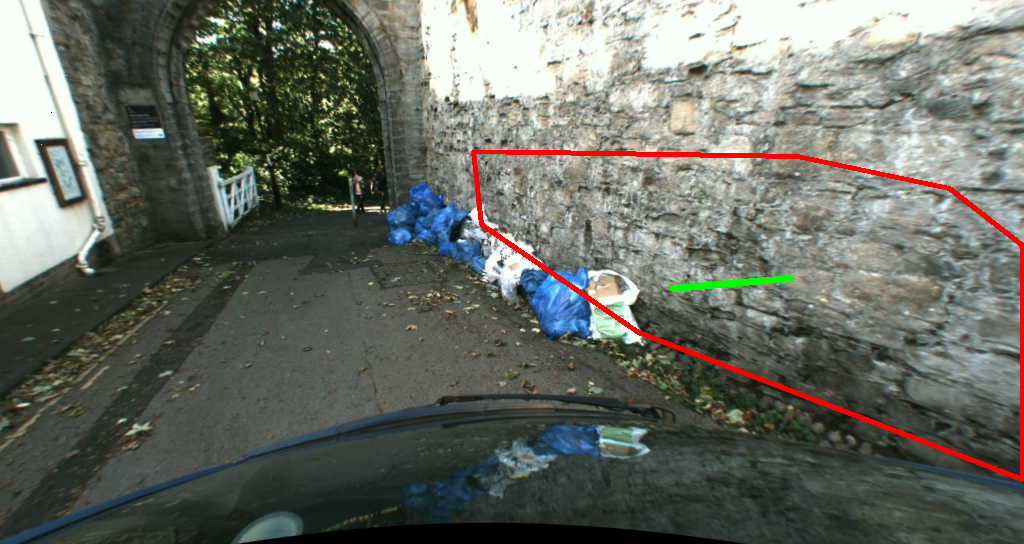
\includegraphics[width=0.4\textwidth]{nob.png}\label{fig:f2}}
        \caption{Results of rejecting RANSAC planes based on y coefficient}
    \end{figure}

\section *{Postprocessing}

\subsection *{Consensus Cleanup}
    The consensus points returned from RANSAC are projected back to 2D, where they are converted to a binary image. Morphology functions can then be used to remove banding effects in the consensus image caused by the discrete nature of the disparity image. Erosion is also performed to remove small areas of consensus separated from the main region.

    \begin{figure}[!h]
        \centering
        \subfloat[Results with cleanup]{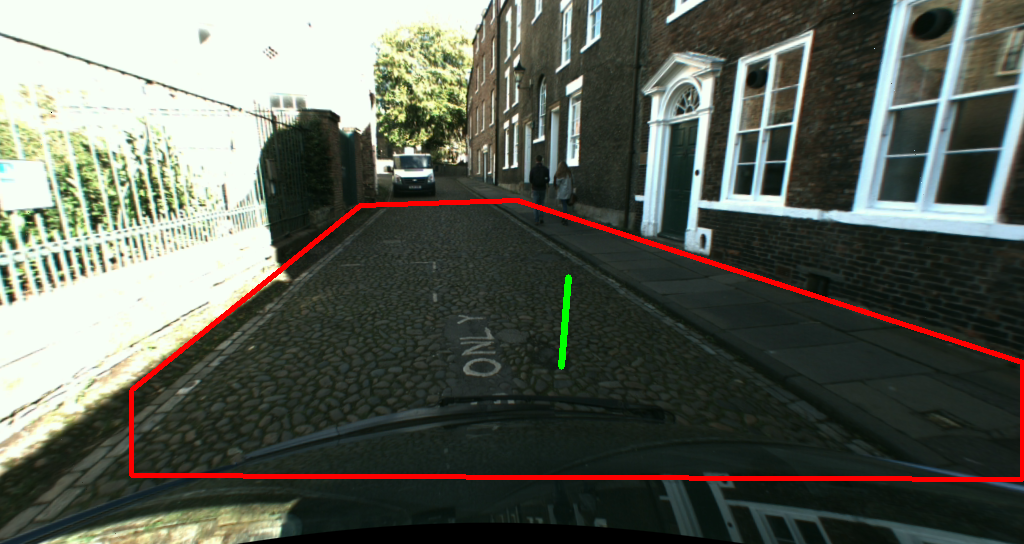
\includegraphics[width=0.4\textwidth]{cleanup.png}\label{fig:f1}}
        \hfill
        \subfloat[Results without cleanup]{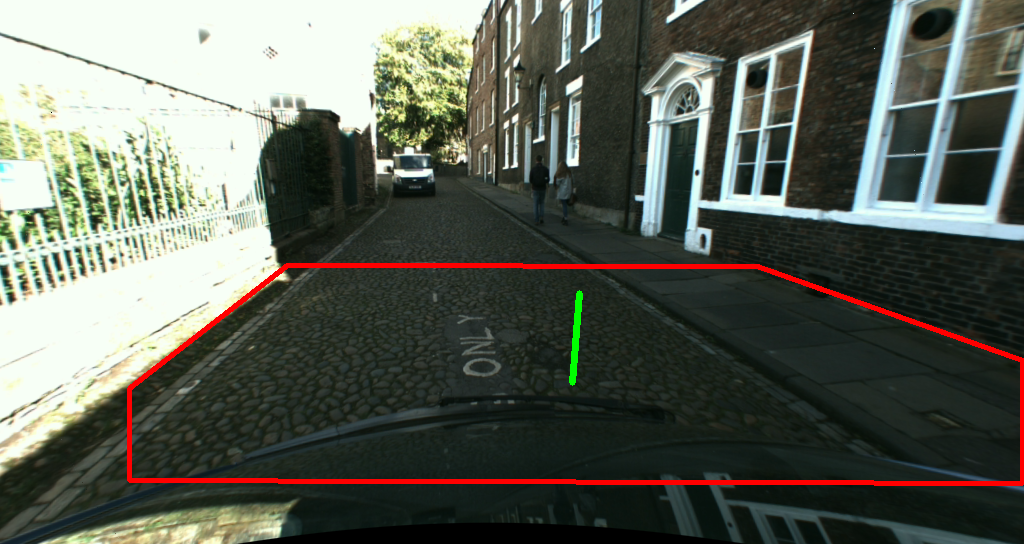
\includegraphics[width=0.4\textwidth]{nocleanup.png}\label{fig:f2}}
        \\
        \subfloat[Consensus with cleanup]{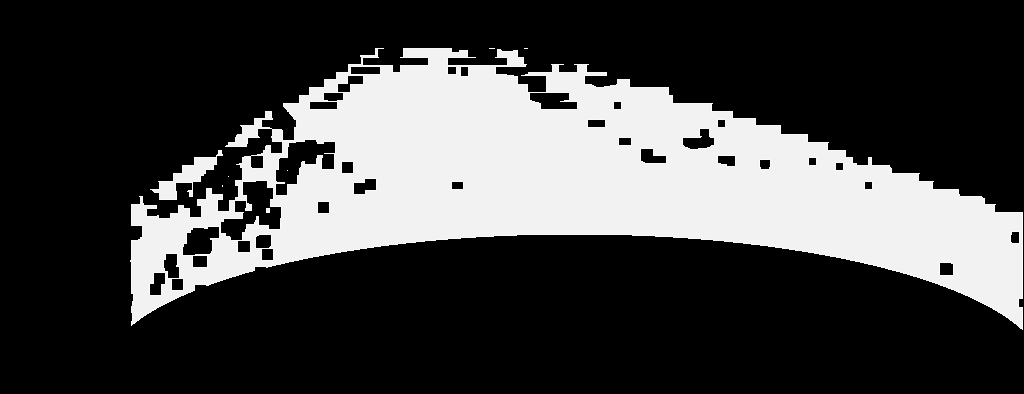
\includegraphics[width=0.4\textwidth]{cleanupcon.png}\label{fig:f1}}
        \hfill
        \subfloat[Consensus without cleanup]{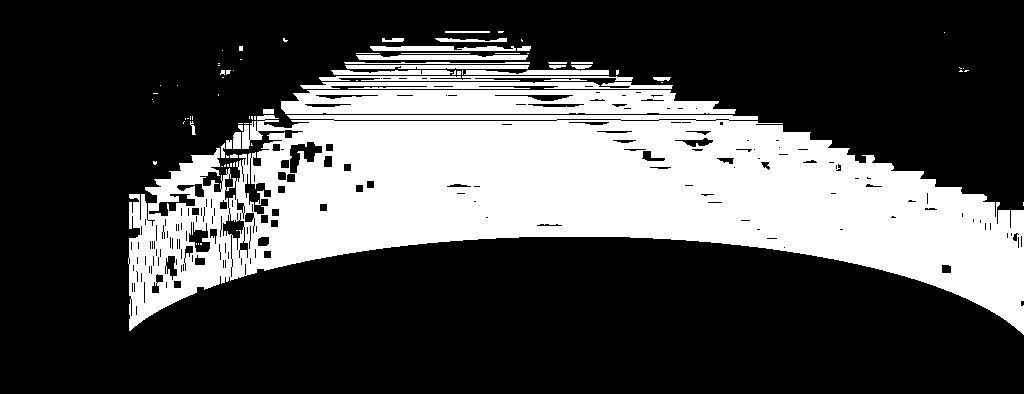
\includegraphics[width=0.4\textwidth]{nocleanupcon.png}\label{fig:f2}}
        \caption{Results of using morphology functions to clean up consensus}
    \end{figure}

\subsection *{Contours}
    Contours of the consensus image are then taken and the road region is defined as the contour with the largest area. The convex hull of this contour is found and approximated to a polygon. This produces more consistent road boundaries at the expense of occasionally ignoring objects on the road's surface such as people and traffic cones.

    \begin{figure}[!h]
        \centering
        \subfloat[With convex hull]{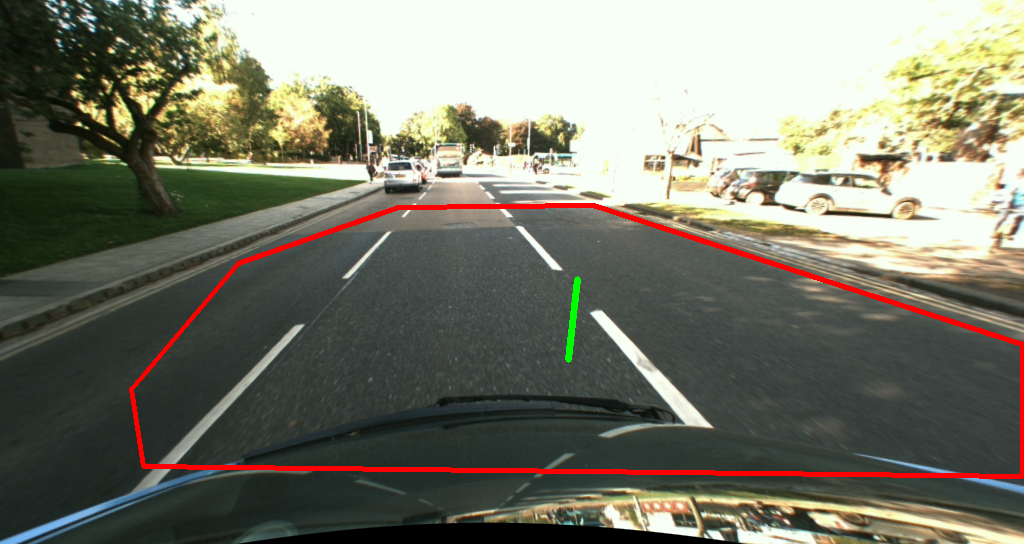
\includegraphics[width=0.4\textwidth]{hull.png}\label{fig:f1}}
        \hfill
        \subfloat[Without convex hull]{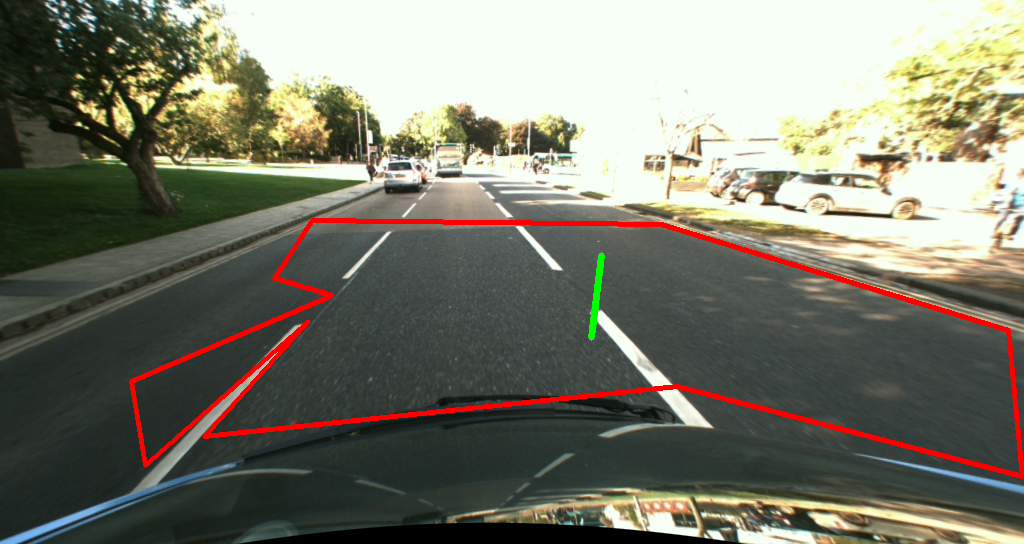
\includegraphics[width=0.4\textwidth]{nohull.png}\label{fig:f2}}
        \\
        \subfloat[With convex hull]{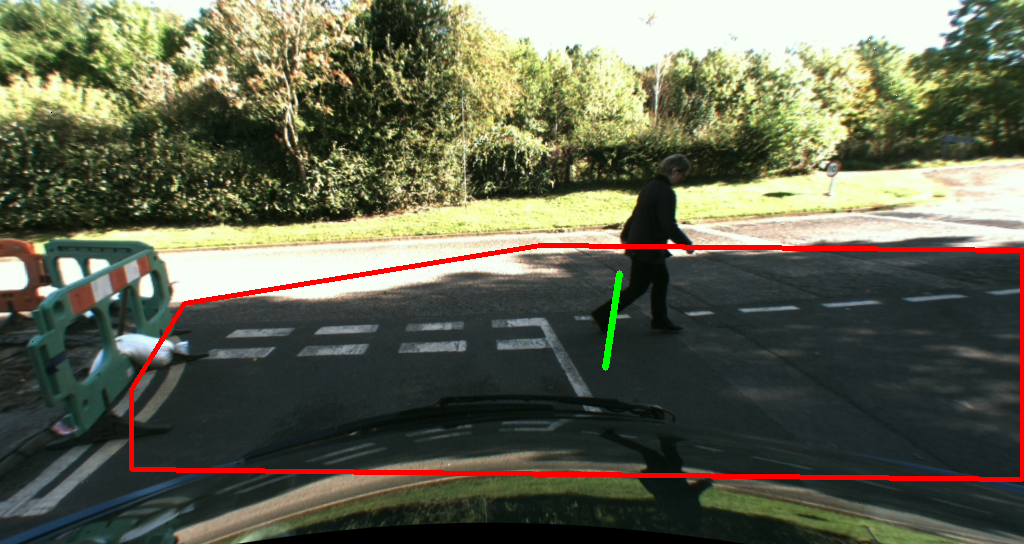
\includegraphics[width=0.4\textwidth]{hull1.png}\label{fig:f1}}
        \hfill
        \subfloat[Without convex hull]{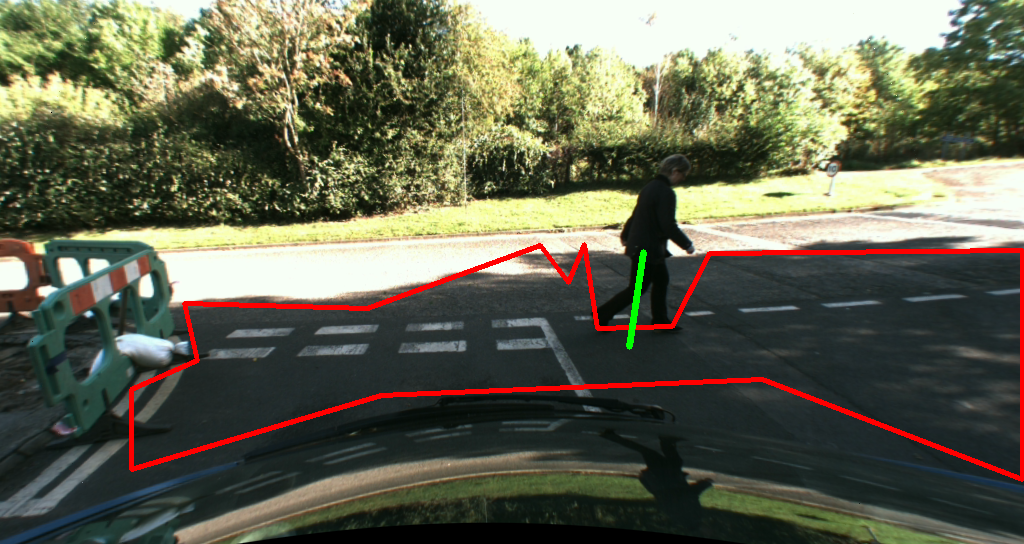
\includegraphics[width=0.4\textwidth]{nohull1.png}\label{fig:f2}}
        \caption{Results of using convex hull to approximate road region}
    \end{figure}

\subsection *{Results}
    Using a random sample of 100 frames, the identified road regions were evaluated in terms of their \textit{coverage} and \textit{purity} where coverage describes the proportion of available road region that was found and purity describes the proportion of the identified region that was in fact road. \\
   \begin{center}
        \begin{tabular}{ r |l | l}
            Score & Coverage & Purity\\
            \hline
            1 & No road found & Contains no road \\
            \hline
            2 & $\approx 25\%$ of road found  & Majority non-road \\
            \hline
            3 & $\approx 50\%$ of road found  & Large areas of non-road\\
            \hline
            4 & $\approx 75\%$ of road found  & Small areas of non-road \\
            \hline
            5 & $\approx 100\%$ of road found & Contains only road\\
        \end{tabular}
    \end{center}


    
    \begin{center}
        \begin{tabular}{ cc|ccccc|c }
            &&\multicolumn{5}{c}{Coverage}&  \\
            && 1 & 2 & 3 & 4 & 5 & Total\\
            \hline
            \parbox[t]{2mm}{\multirow{5}{*}{\rotatebox[origin=c]{90}{Purity}}}&1& 1 & 0 & 0 & 0 & 0 & 1\\
            &2 & 1& 0 & 0 & 2 & 4 & 7\\
            &3& 1& 1 & 2 & 8 & 6 & 18\\
            &4&0 & 2 & 7 & 7 & 16 & 32 \\
            &5 & 0 & 2 & 10 & 15 & 15 & 42 \\
            \hline
            Total & & 3 & 5 & 19 & 32 & 41 &  \\


        \end{tabular}
    \end{center}

    \noindent From this sample, the mean score was 4.03 for coverage and 4.07 for purity. This indicates that on average, a large proportion of road will be successfully identified with only a small area of the identified region being a false positive.
    \begin{figure}[!h]
        \centering
        \subfloat[coverage=1 purity=1]{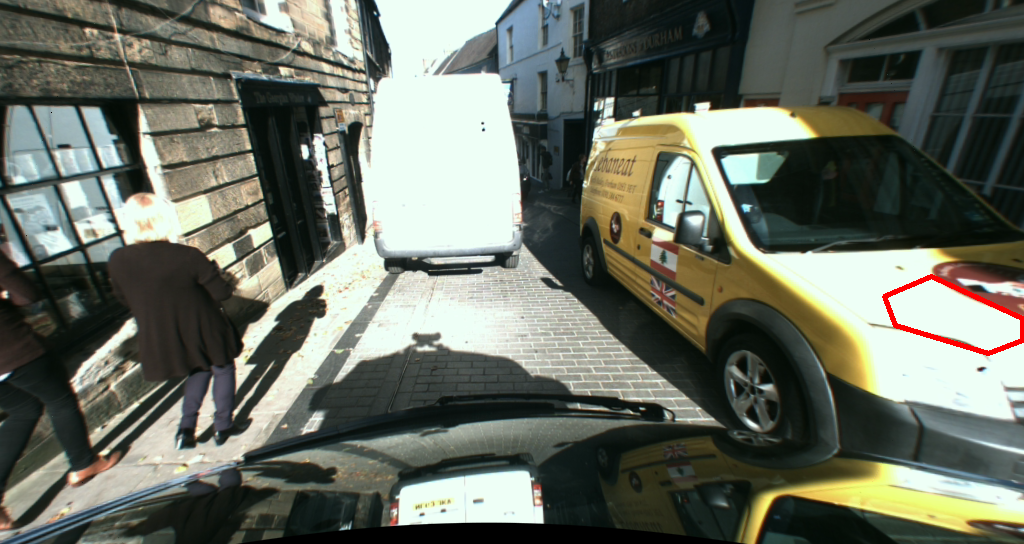
\includegraphics[width=0.4\textwidth]{11.png}\label{fig:f1}}
        \hfill
        \subfloat[coverage=2 purity=3]{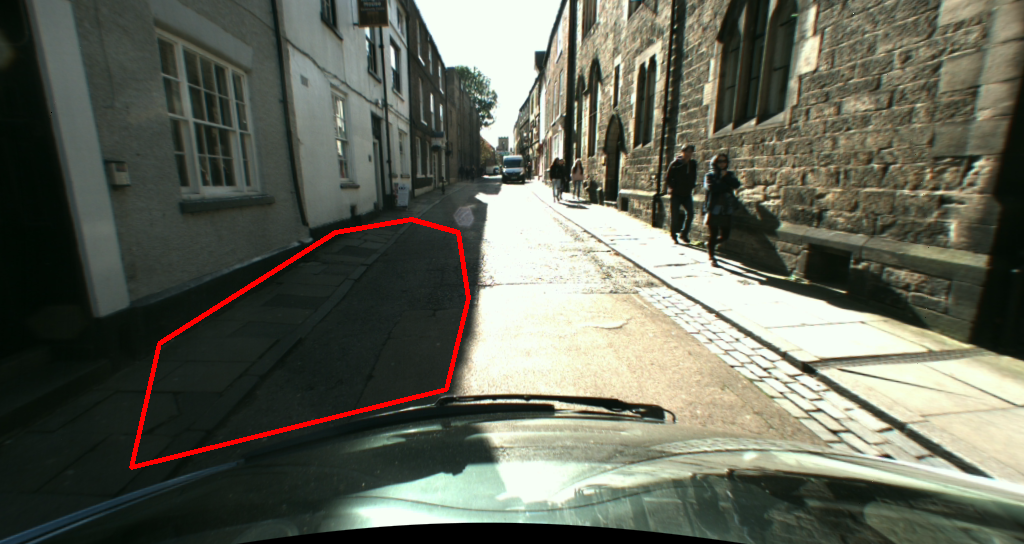
\includegraphics[width=0.4\textwidth]{23.png}\label{fig:f1}}
        \\
        \subfloat[coverage=3 purity=3]{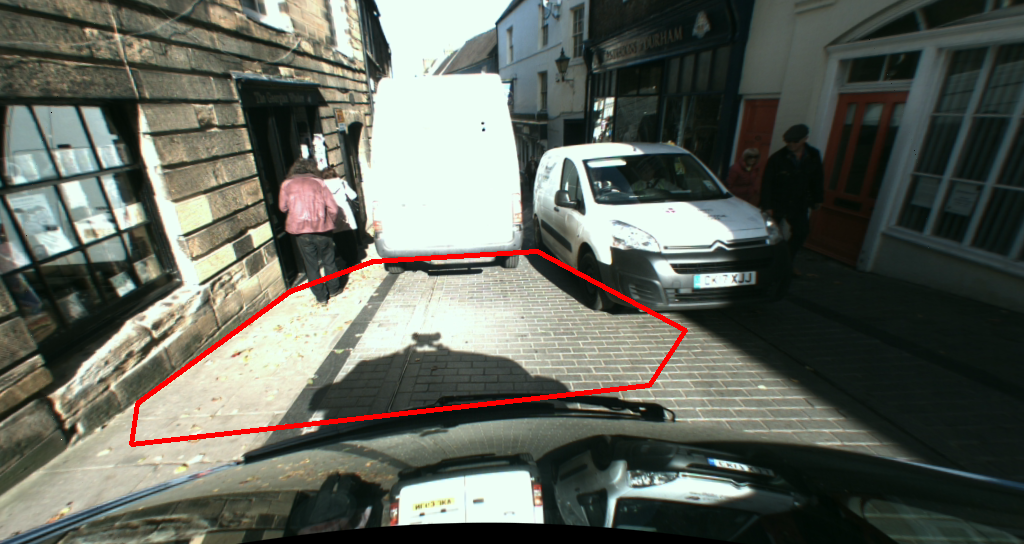
\includegraphics[width=0.4\textwidth]{33.png}\label{fig:f1}}
        \hfill
        \subfloat[coverage=4 purity=4]{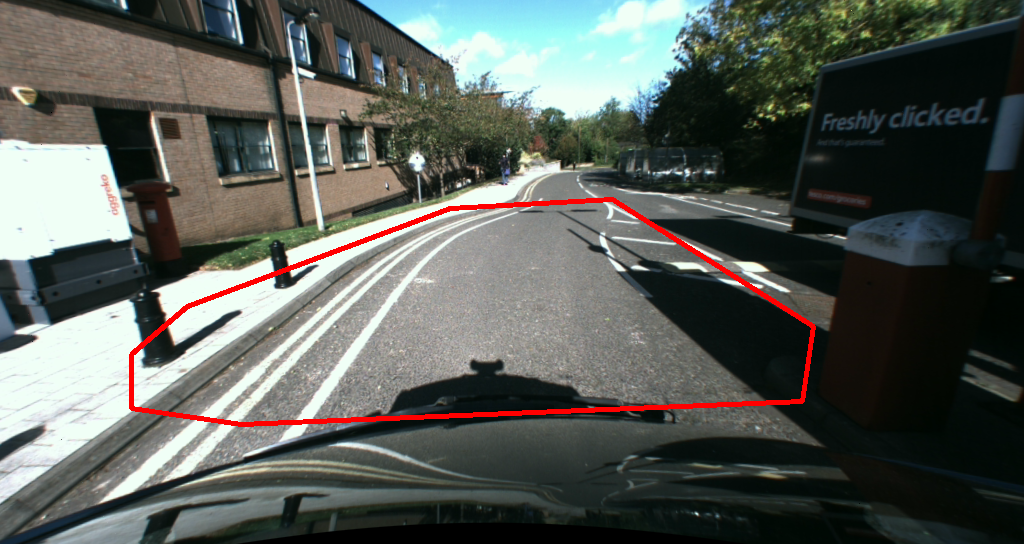
\includegraphics[width=0.4\textwidth]{44.png}\label{fig:f1}}
        \\
        \subfloat[coverage=5 purity=5]{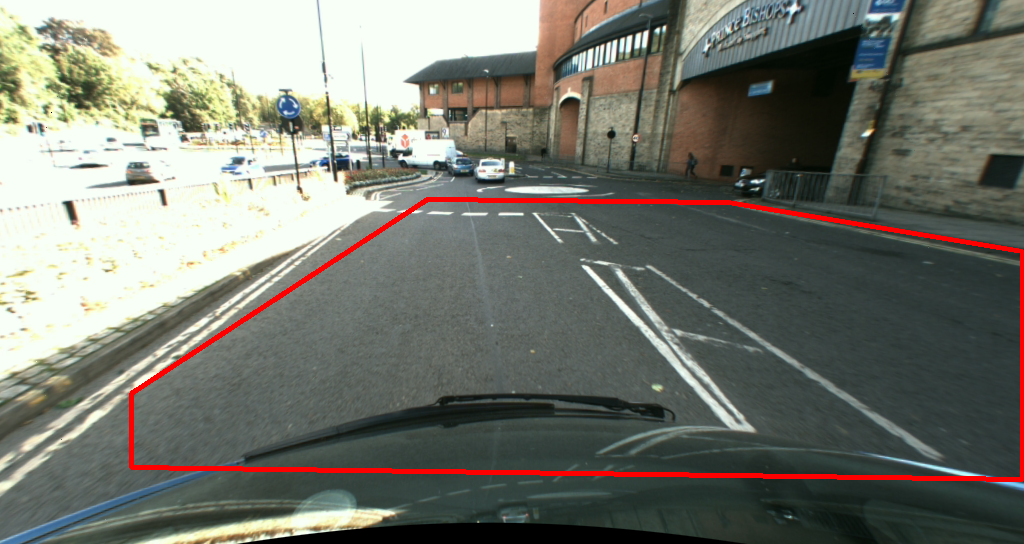
\includegraphics[width=0.4\textwidth]{55.png}\label{fig:f1}}
        \hfill
        \subfloat[coverage=5 purity=2]{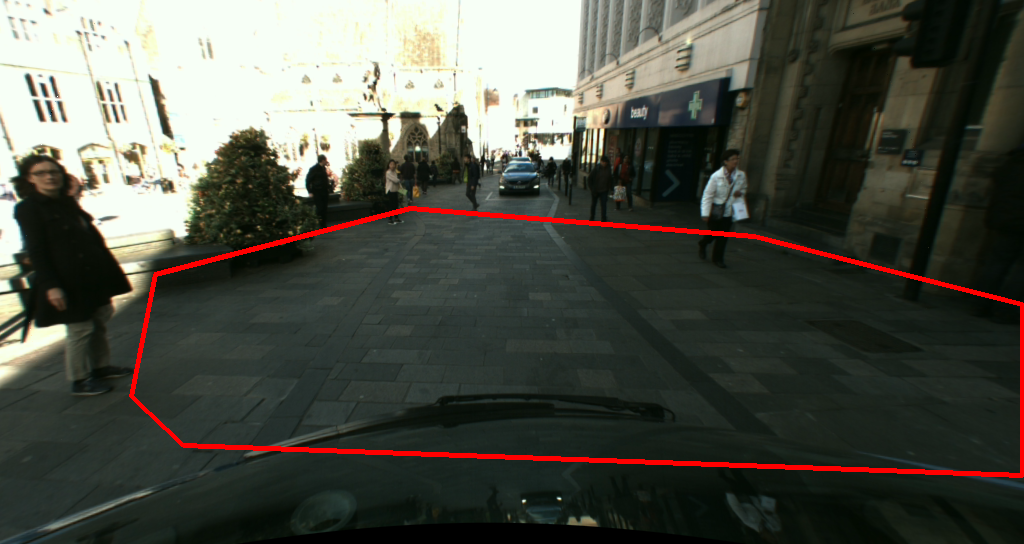
\includegraphics[width=0.4\textwidth]{52.png}\label{fig:f1}}
        \caption{Sample of result images used in evaluation}
    \end{figure}
    
\printbibliography
% 
 

\end{document} 